\chapter{Reinforcement Learning}
\begin{quotation}
\noindent ``\emph{quote}''
\begin{flushright}\textbf{auteur, date}\end{flushright}
\end{quotation}

\vspace*{0.5cm}

\section{The reinforcement learning problem}
A reinforcement learning setting sees two main components interact : the agent
and the environment. The environment can be in several states which the agent
can observe (for example in the CartPole problem : the cart can be in several 
positions and have different velocities, and the pole has similar 
characteristics). In some problems, the agent might not be able to observe the
full state of the environment.\\

The agent chooses actions based on its knowledge of the state of the
environment. These actions might (and often do) alter the state of the
environment, but will also generate a reward. In the CartPole problem, the 
reward is +1 every tick the pole is above a certain angle, 0 otherwise.\\

With this simple setting, of which a diagram is shown in Figure~\ref{fig:rl},
we can design algorithms that can be trained to solve a huge variety of tasks
without ever having to include task-specific logic to the algorithm.

\begin{figure}[]
	\centering
	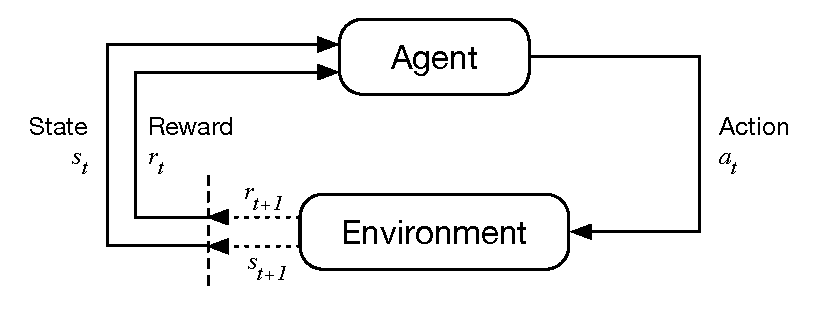
\includegraphics[width=0.65\linewidth]{fig/rl.eps}
	\caption{The setting of a reinforcement learning problem 
		\cite{suttonbarto}}
	\label{fig:rl}
\end{figure}

\subsection{Markov Decision Processes}
A reinforcement learning problem can be formally defined as a Markov 
Decision Process (MDP) \index{MDP} characterised by :
\begin{itemize}
	\item a set of states $\mathcal{S}$
	\item a set of actions $\mathcal{A}$
	\item a transition function 
		$T(s, a, s') = P(s_{t+1} = s' \mid s_t = s, a_t = a)$
	\item a reward function 
		$r(s, a, s') = \mathbb{E}
		 [r_{t+1} \mid s_t = s, a_t = a, s_{t+1} = s']$
\end{itemize}
For the rest of this paper, we will consider that the transition function is
deterministic.\\

The goal of reinforcement learning is for the agent to select, in any state it
can be in, the action that will lead it to the highest expected reward :

\begin{equation}
\label{eq:discounted_reward}
\mathbb{E}[r] = R_t = r_t + \gamma r_{t+1} + \gamma^2 r_{t+2}^2 + ... =
 \sum\limits_{i=0}^\infty \gamma^i r_{t+i}
\end{equation}

\noindent with the discount factor \index{discount factor} $\gamma \in [0, 1[$.
The discount factor allows one to tune the agent's behaviour on the
short-term/long-term spectrum. A discount factor $\gamma=0$ would mean that the
agent maximises its expected reward for the next transition only whereas a
discount factor close to one will favour behaviour that maximises long-term
reward, even if one action leads to a poor reward at first.\\

\subsection{Policy}
The agent uses a policy $\pi(a \mid s)$ which describes a probability
distribution over the action set $\mathcal{A}$, determining the probability of
selecting action $a_i$ from state $s_i$. This policy is 
\textbf{deterministic} if and only if :
\begin{equation}
\forall\, s \in \mathcal{S},\; \exists\, a \in \mathcal{A} : \pi(a \mid s) = 1
\end{equation}
\noindent In other words : in any state, only one action can be selected.
Otherwise, the policy is \textbf{stochastic}.

\section{An example : the 2-armed bandit problem}
The 2-armed bandit setting defines two actions that the agent can perform,
each of which associated with one arm. Each arm has an underlying reward
distribution -- for the sake of this example, let us define each arm with the
following Bernoulli distributions: 

\begin{table}[H]
	\centering
	\begin{tabular}{c|c}
		Arm \#1 & Arm \#2 \\ \hline
		0.9 & 0.1
	\end{tabular}
\end{table}

\noindent This means that arm \#1 will generate a reward of 1 with a probability
of 0.9 and arm \#2 will generate a reward of 1 with a probability of 0.1.\\

The careful reader will have noticed that this problem is stateless 
($\mathcal{S} = \{\varnothing\}$), meaning that the agent only perceives
rewards and no state observations.\\

Of course, before its first interaction with the environment, the agent has no
information whatsoever about the reward distribution of each arm, and the whole
idea of reinforcement learning is to look for evermore efficient ways to learn
the structure and parameters of a problem in order to maximise reward.\\

One could imagine a simple strategy like the following : play each arm 10 times,
then always play the arm with the highest average reward. This policy is
deterministic, and yields either $ \pi(a_1) = 1$ and $\pi(a_2) = 0$ or
$\pi(a_1) = 0$ and $\pi(a_2) = 1$. This could work in
our case, but might fail in cases where the distributions are much closer
(e.g. 0.45 and 0.55). What if the reward was sampled out of overlapping normal
distributions?\\

Deciding whether the following action should be used to explore the environment
and gain information about it; or to exploit the information already available
to try to maximise reward is not trivial. Exploring could make training slower
or affect the reward if our model of the environment is correct, but it is 
needed to increase the probability that we have indeed a correct model. This
tradeoff is called the exploration/exploitation tradeoff. 




